\documentclass[10pt,twocolumn,letterpaper]{article}

\usepackage{cvpr}
\usepackage{times}
\usepackage{epsfig}
\usepackage{graphicx}
\usepackage{amsmath}
\usepackage{amssymb}
\usepackage{float} 
\usepackage{subfigure} 
\usepackage{bm} 
\usepackage{algorithm}
\usepackage{tabularx}
\usepackage{algpseudocode}
\usepackage{subfloat}
\usepackage{verbatim}


\usepackage[pagebackref=true,breaklinks=true,letterpaper=true,colorlinks,bookmarks=false]{hyperref}
\usepackage[american]{babel}
\usepackage{microtype}

\hypersetup{
    colorlinks=true,
    linkcolor=blue,
    filecolor=red,      
    urlcolor=red,
    citecolor=green,
}

\makeatletter
\usepackage{xspace}
\DeclareRobustCommand\onedot{\futurelet\@let@token\@onedot}
\def\@onedot{\ifx\@let@token.\else.\null\fi\xspace}
\def\eg{\emph{e.g}\onedot}
\def\ie{\emph{i.e}\onedot}
\def\etal{\emph{et al}\onedot}
\makeatother

\def\cvprPaperID{6791}

\def\httilde{\mbox{\tt\raisebox{-.5ex}{\symbol{126}}}}

\renewcommand{\algorithmicrequire}{\textbf{Input:}}
\renewcommand{\algorithmicensure}{\textbf{Output:}}

\begin{document}

\bibliographystyle{plain}

\title{Learning to Cartoonize Using White-box Cartoon Representations}
\maketitle
\begin{abstract}

This paper presents an approach for image cartoonization. By observing the cartoon painting behavior and consulting artists, we propose to separately identify three white-box representations from images: the surface representation that contains smooth surface of cartoon images, the structure representation that refers to the sparse color-blocks and flatten global content in the celluloid style workflow, and the texture representation that reflects high-frequency texture, contours and details in cartoon images. A Generative Adversarial Network (GAN) framework is used to learn the extracted representations and to cartoonize images. 

The learning objectives of our method are separately based on each extracted representations, making our framework controllable and adjustable. This enables our approach to meet artists' requirements in different styles and diverse use cases. Qualitative comparisons and quantitative analyses, as well as user studies, have been conducted to validate the effectiveness of this approach, and our method outperforms previous methods in all comparisons. Finally, the ablation study demonstrates the influence of each component in our framework. 

\begin{comment}
Controllable and tunable white-box representations enable our approach to meet artists' requirements in diverse use cases. Besides, the clear and independent learning objective for separate representations significantly improves the visual quality of cartoonized results, making the output style adjustable. Qualitative comparisons and quantitative analyses, as well as user studies, have been conducted to validate the effectiveness of this approach. Finally, the ablation study demonstrates the influence of each component in our framework. 
\end{comment}
\end{abstract}
\vspace{-1em}
\section{Introduction}
%\vspace{-0.5em}
Cartoon is a popular artistic form that has been widely applied in diverse scenes. Modern cartoon animation workflows allow artists to use a variety of sources to create contents. Some famous products have been created by turning real-world photography into usable cartoon scene materials, where the process is called image cartoonization.
\begin{figure}[t]
\centering
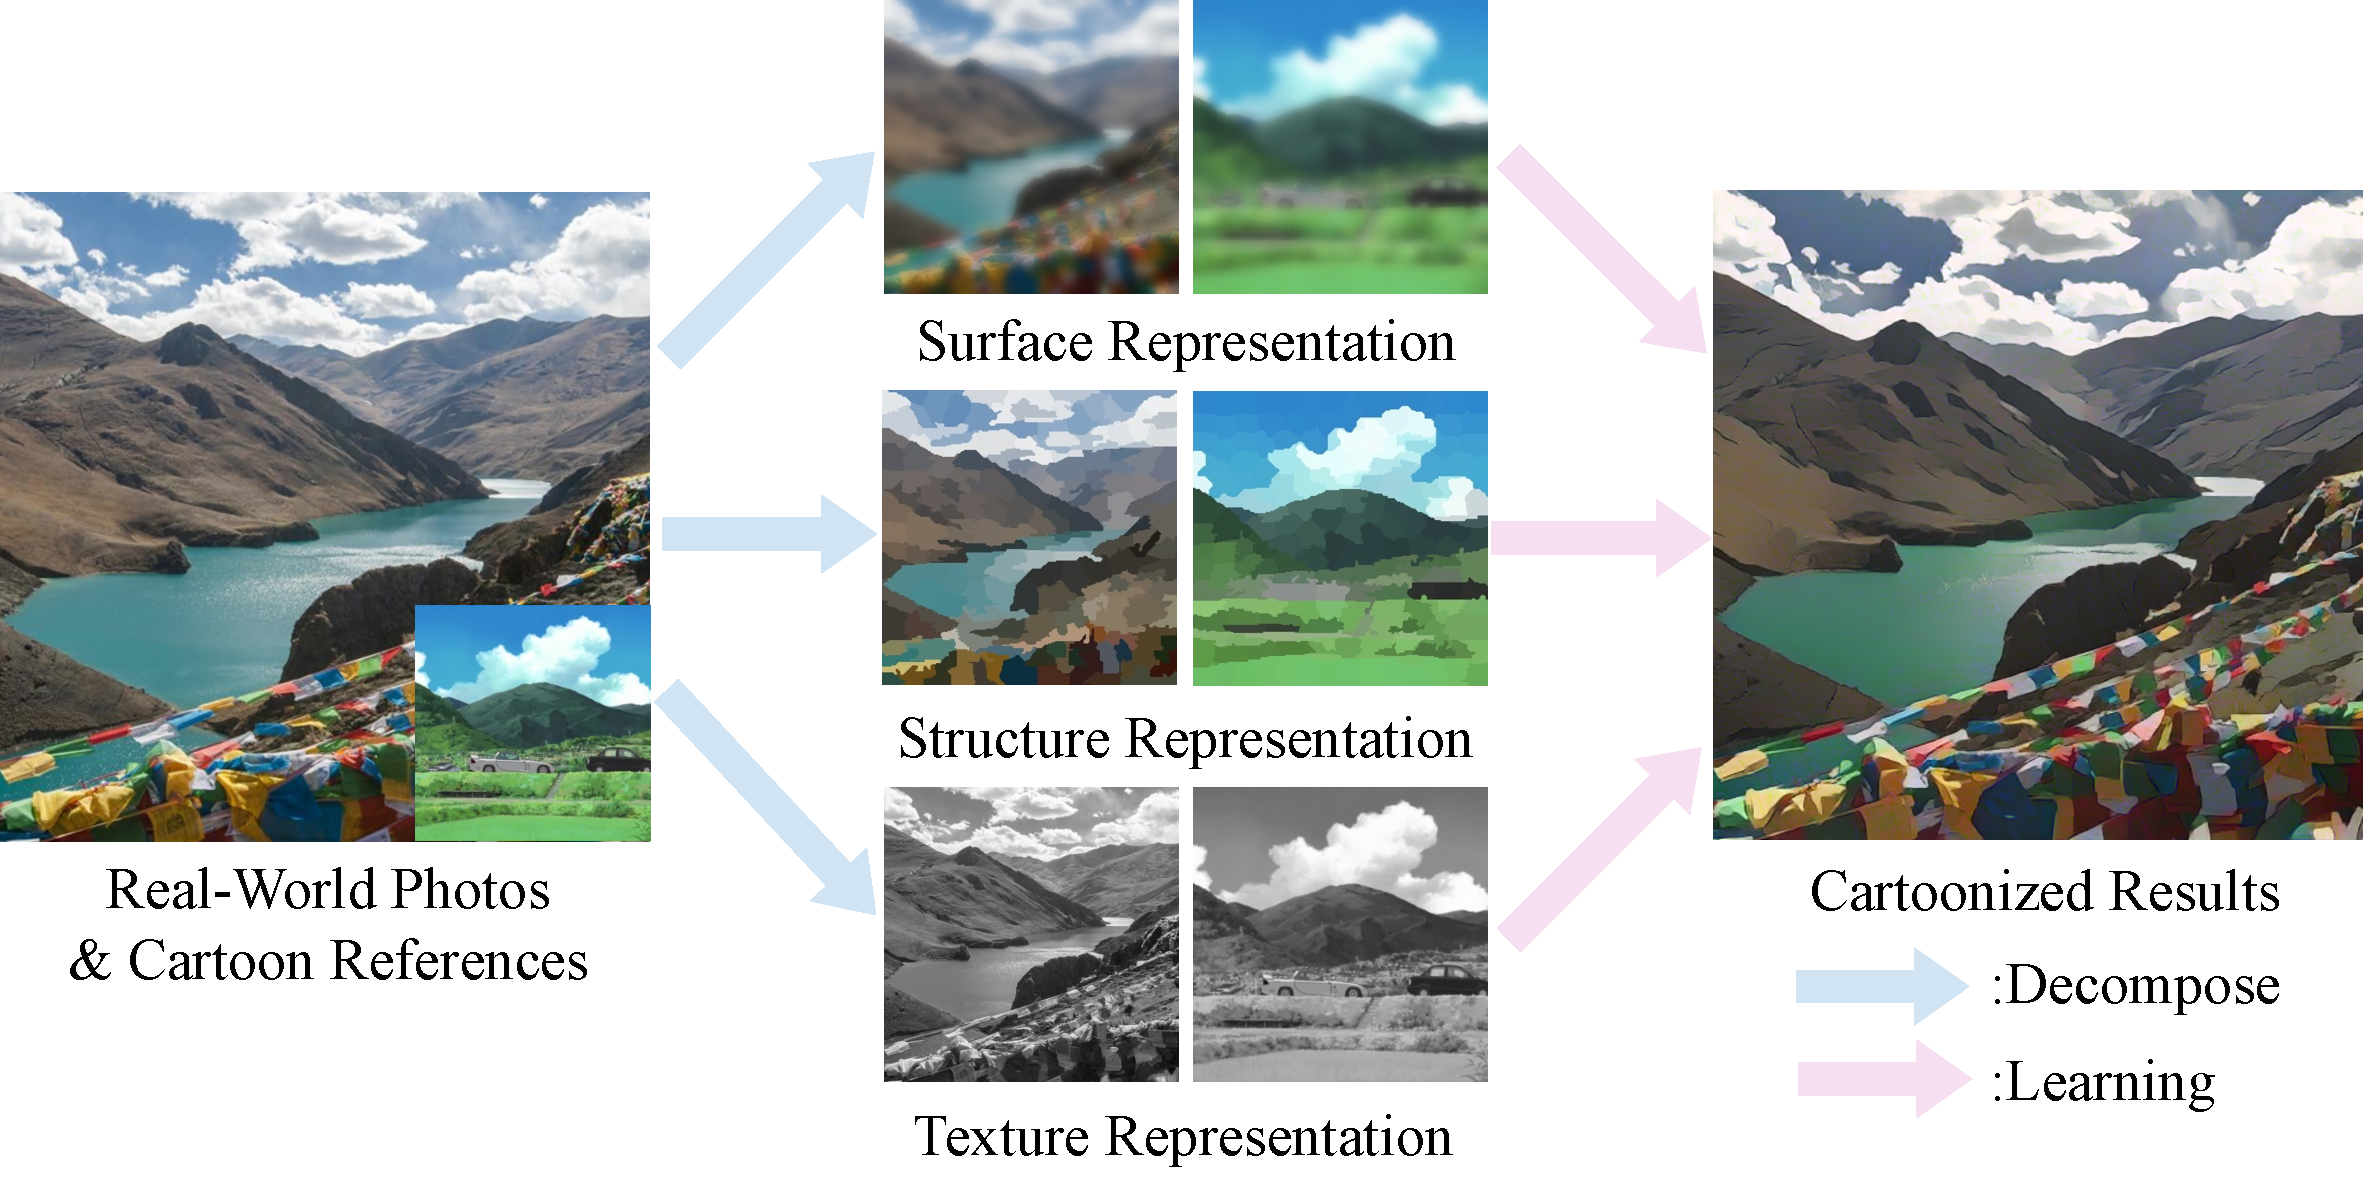
\includegraphics[width=\linewidth]{imgs/figure1}
\caption{A simple illustration of our method. Images are decomposed into three cartoon representations, which guide the network optimization to generate cartoonized real-world photos.}
\label{fig:shinjuku}
\vspace{-1em}
\end{figure}

The variety of cartoon styles and use cases require task-specific assumptions or prior knowledge to develop usable algorithms. For example, some cartoon workflows pay more attention to global palette themes, but the sharpness of lines is a secondary issue. In some other workflows, sparse and clean color blocks play a dominant role in artistic expression, but the themes are relatively less emphasized. 

These variants pose non-trivial challenges to black-box end-to-end models, \eg, \cite{johnson2016perceptual, CycleGAN2017, chen2018cartoongan}, when faced with diverse demands of artists in different use cases, and simply change the training dataset does not help. Especially, CartoonGAN \cite{chen2018cartoongan} is designed for image cartoonization, in which a GAN framework with a novel edge loss is proposed, and achieves good results in certain cases. But using black-box model to directly fit the training data decreased its generality and stylization quality, causing bad cases in some situations. 

To address the above-mentioned problems, we made extensive observations on human painting behaviors and cartoon images of different styles, and also consulted several cartoon artists. According to our observations, which is shown in Figure \ref{fig:representation}, we propose to decompose images into several cartoon representations, and list them as follows:

Firstly, we extract the \emph{surface} representation to represent the smooth surface of images. Given an image $\bm{I} \in \mathbb{R}^{W \times H \times 3}$, we extract a weighted low-frequency component $\bm{I}_{sf} \in \mathbb{R}^{W \times H \times 3}$, where the color composition and surface texture are preserved with edges, textures and details ignored. This design is inspired by the cartoon painting behavior where artists usually draw composition drafts before the details are retouched, and is used to achieve a flexible and learnable feature representation for smoothed surfaces.

Secondly, the \emph{structure} representation is proposed to effectively seize the global structural information and sparse color blocks in celluloid cartoon style. We extract a segmentation map from the input image $\bm{I} \in \mathbb{R}^{W \times H \times 3}$ and then apply an adaptive coloring algorithm on each segmented regions to generate the structure representation $\bm{I}_{st} \in \mathbb{R}^{W \times H \times 3}$. This representation is motivated to emulate the celluloid cartoon style, which is featured by clear boundaries and sparse color blocks. The structure representation is of significance for generating the sparse visual effects, as well as for our method to be embedded in the celluloid style cartoon workflow.

Thirdly, we use the \emph{texture} representation to contain painted details and edges. The input image $\bm{I} \in \mathbb{R}^{W \times H \times 3}$ is converted to a single-channel intensity map $\bm{I}_{t} \in \mathbb{R}^{W \times H \times 1}$, where the color and luminance are removed and relative pixel intensity is preserved. This feature representation is motivated by a cartoon painting method where artists firstly draw a line sketch with contours and details, and then apply color on it. It guides the network to learn the high-frequency textural details independently with the color and luminance patterns excluded.
\begin{figure}[t]
\centering
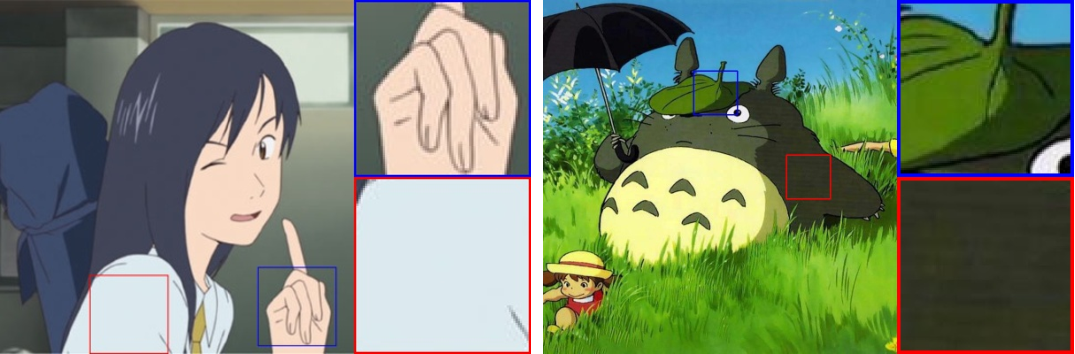
\includegraphics[width=\linewidth]{imgs/representation.pdf}
\caption{Cartoon images with some typical and common features: 1. Global structures are composed of sparse color blocks and clear boundaries; 2. Details are outlines by sharp and clear contours; 3. Surfaces are flat and smooth.}
\label{fig:representation}
\vspace{-1em}
\end{figure}

It is worth noting that the extractions of the surface representation and the texture representation are differentiable, which enables the cartooniaztion problem to be optimized end-to-end within a Generative Neural Networks (GAN) framework. Moreover, the separated cartoon representations make our method scalable and controllable for practical use cases and easy to meet diversified artistic demands with task-specific fine-tuning. 

We apply our method on a variety of real-world photos on diverse scenes and generate their cartoonized counterparts in different styles. Experimental results show that our method can generate images with harmonious color, pleasing artistic styles, sharp and clean boundaries, and significantly fewer artifacts as well. We also show that our method outperforms previous state-of-the-art methods through qualitative experiments, quantitative experiments, and user studies. Finally, ablation studies are also conducted to illustrate the influence of each cartoon representations. To conclude, our contributions are summarized as follows:

\begin{itemize}
\setlength{\itemsep}{0.5pt}
\setlength{\parsep}{0pt}
\setlength{\parskip}{0pt}
\item We propose three cartoon representations based on our observation of cartoon painting behavior: the surface representation, the structure representation, and the texture representation. Image processing modules are then introduced to extract each representation.
\item A GAN-based controllable image cartoonization framework is optimized with the guide of extracted representations. Users can adjust the style of model output by balancing the weight of each representation.
\item Extensive experiments have been conducted to show that our method can generate high-quality cartoonized images. Our method outperforms existing methods in qualitative comparison, quantitative comparison, and user preference.
\end{itemize}
\vspace{-0.3em}
\section{Related Work}
\vspace{-0.3em}
\subsection{Image Smoothing and Surface Extraction}
Image smoothing~\cite{tomasi1998bilateral, he2010guided, farbman2008edge, min2014fast, bi20151} is an extensively studied topic. Early methods are mainly filtering based~\cite{tomasi1998bilateral, he2010guided} and optimization-based methods later became popular. Farbman~\etal~\cite{farbman2008edge} utilized weighted least square to constrain the edge-preserving operator, Min~\etal~\cite{min2014fast} solved global image smoothing by minimizing a quadratic energy function, and Bi~\etal~\cite{bi20151} proposed a L1 transformation for image smoothing and flattening problem. Xu and Fan~\etal~\cite{xu2015deep, fan2017generic, fan2018image} introduced end-to-end networks for image smoothing. In this work, we adapt a differentiable guided filter \cite{wu2018fast} to extract smooth, cartoon-like surface from images, enabling our model to learn structure-level composition and smooth surface that artists have created in cartoon artworks.
 
\begin{figure*}[t]
\centering
\includegraphics[width=\linewidth]{imgs/method.pdf}
\caption{Our proposed image cartoonization system}
\label{fig:framework}
\vspace{-1em}
\end{figure*}

\vspace{-0.3em}
\subsection{Superpixel and structure Extraction}
\vspace{-0.3em}
Super-pixel segmentation \cite{felzenszwalb2004efficient, mori2005guiding, moore2008superpixel, achanta2012slic, levinshtein2009turbopixels} groups spatially connected pixels in an image with similar color or gray level. Some popular super-pixel algorithms \cite{felzenszwalb2004efficient, mori2005guiding, moore2008superpixel} are graph-based, treating pixels as nodes and similarity between pixels as edges in a graph. Gradient ascent based algorithms \cite{comaniciu2002mean, vedaldi2008quick, achanta2012slic,  levinshtein2009turbopixels} initialize the image with rough clusters and iteratively optimize the clusters with gradient ascent until convergence. In this work, we follow the felzenszwalb algorithm \cite{felzenszwalb2004efficient} to develop a cartoon-oriented segmentation method to achieve a learnable structure representation. This representation is significant for deep models to seize global content information and produce practically usable results for celluloid style cartoon workflows.

\vspace{-0.3em}
\subsection{Non-photorealistic Rendering and Neural Style Transfer}
\vspace{-0.3em}
Non-photorealistic Rendering (NPR) methods represent image content with artistic styles, such as pencil sketching \cite{xu2011image, lu2012combining}, paints \cite{gatys2015neural, johnson2016perceptual}, watercolor \cite{van2004real, curtis1997computer}. Image cartoonization is also extensively studied from filtering based method \cite{shahcheraghi2013effects} to end-to-end neural network \cite{chen2018cartoongan}, covering the use cases of photos \cite{chen2018cartoongan}, videos \cite{wang2004video}, and portraits \cite{rosin2015non, yang2010semantics}.

Neural Style Transfer methods \cite{gatys2015neural, johnson2016perceptual, dumoulin2016learned, huang2017arbitrary, li2017universal} are popular among NPR algorithms, which synthesis images with artistic style by combining the content of one image and the style of another image. Gatys~\etal~\cite{gatys2015neural} jointly optimized a style loss and a content loss to generate stylize images with a style-content image pair. Johnson \etal \cite{johnson2016perceptual} accelerated this process by training an end-to-end network with perception loss. Several works \cite{dumoulin2016learned, huang2017arbitrary, li2017universal} later proposed models to synthesis images with different styles. Our method, different from the above-mentioned methods that take a single image as a style, learns the cartoon data distribution from a set of cartoon images. This allows our model to synthesis high-quality cartoonized images on diverse use cases.
\vspace{-0.3em}
\subsection{Generative Adversarial Networks}
\vspace{-0.3em}
Generative Adversarial Network(GAN) \cite{goodfellow2014generative} is a state-of-the-art generative model that can generate data with the same distribution of input data by solving a min-max problem between a generator network and a discriminator network. It is powerful in image synthesis by forcing the generated images to be indistinguishable from real images. GAN has been widely used in conditional image generation tasks, such as image inpainting \cite{pathak2016context}, style transfer \cite{sanakoyeu2018style}, image cartoonization \cite{chen2018cartoongan}, image colorization \cite{zhang2018two}. In our method, we adopt adversarial training architecture and use two discriminators to enforce the generator network to synthesis images with the same distribution as the target domain.
\vspace{-0.3em}
\subsection{Image-to-Image Translation}
\vspace{-0.3em}
Image-to-Image Translation \cite{isola2017image, huang2018multimodal, lee2018diverse, CycleGAN2017} tackles the problem of translating images from a source domain to another target domain. Its applications include image quality enhancement \cite{ignatov2018wespe}, stylizing photos into paints \cite{johnson2016perceptual, sanakoyeu2018style}, cartoon images \cite{chen2018cartoongan} and sketches \cite{li2019im2pencil}, as well as grayscale photo colorization \cite{zhang2016colorful} and sketch colorizaiton \cite{zhang2018two}. Recently,  bi-directional models are also introduced for inter-domain translation. Zhu \etal \cite{CycleGAN2017} performs transformation of unpaired images(i.e. summer to winter, photo to paints). 

In this paper, we adopt an unpaired image-to-image translation framework for image cartoonization. Unlike previous black-box models that guide network training with loss terms, we decompose images into several representations, which enforces network to learn different features with separate objectives, making the learning process controllable and tunable. 

\vspace{-0.3em}
\section{Proposed Approach}
\vspace{-0.3em}
We show our proposed image cartoonizaiton framework in Figure \ref{fig:framework}. Images are decomposed into the surface representation, the structure representation, and the texture representations, and three independent modules are introduced to extract corresponding representations. A GAN framework with a generator $\textit G$ and two discriminators $\textit D_{s}$ and $\textit D_{t}$ is proposed, where $\textit D_{s}$ aims to distinguish between surface representation extracted from model outputs and cartoons, and $\textit D_{t}$ is used to distinguish between texture representation extracted from outputs and cartoons. Pre-trained VGG network \cite{simonyan2014very} is used to extract high-level features and to impose spatial constrain on global contents between extracted structure representations and outputs, and also between input photos and outputs. Weight for each component can be adjusted in the loss function, which allows users to control the output style and adapt the model to diverse use cases.
\vspace{-0.3em}
\subsection{Learning From the Surface Representation}
\vspace{-0.3em}
The surface representation imitates cartoon painting style where artists roughly draw drafts with coarse brushes and have smooth surfaces similar to cartoon images. To smooth images and meanwhile keep the global semantic structure, a differentiable guided filter is adopted for edge-preserving filtering. Denoted as $\mathcal{F}_{dgf}$,  it takes an image $\bm{I}$ as input and itself as guide map, and returns extracted surface representation $\mathcal{F}_{dgf}(\bm{I}, \bm{I})$ with textures and details removed. 

 A discriminator $D_{s}$ is introduced to judge whether model outputs and reference cartoon images have similar surfaces, and guide the generator $G$ to learn the information stored in the extracted surface representation. Let $\bm{I_p}$ denote the input photo and $\bm{I_c}$ denote the reference cartoon images, we formulate the surface loss as:
\begin{equation}
\vspace{-0.5em}
\begin{aligned}
\mathcal{L}_{surface}(\textit G,~&\textit D_{s}) = log\textit D_{s}({\mathcal{F}_{dgf}}(\bm{I}_c, \bm{I}_c))\\
&+log(1-\textit D_{s}(\mathcal{F}_{dgf}(\textit G(\bm{I}_p), \textit G(\bm{I}_p))))
\end{aligned}
\label{eqn:equation1}
\end{equation}

\vspace{-0.3em}
\subsection{Learning From the Structure representation}
\vspace{-0.3em}
The Structure representation emulates flatten global content, sparse color blocks and clear boundaries in celluloid style cartoon work-flow. We at first use felzenszwalb algorithm to segment images into separate regions. As superpixel algorithms only consider the similarity of pixels and ignore semantic information, we further introduce selective search \cite{uijlings2013selective} to merge segmented regions and extract a sparse segmentation map $\bm{T}$. Denoted as $\mathcal{F}_{seg}$, the segmentation algorithm is described in Algorithm \ref{alg:algorithmic1}. For the similarity metric, we consider both pixel value and spatial coordinate, and defined it as the euclidean distance in (x, y, l, a, b) 5 dimension space, where x and y represent coordinates and l, a, b represent pixel value in LAB color space.

\vspace{-0.5em}
\begin{algorithm}
     \caption{Segmentation for the Structure Representation}
    \begin{algorithmic}[1]
     \Require  ~~~Input image $\bm{I}$, number of regions $\bm{N}$
     \Ensure Extracted segmentation map $\bm{T} = \mathcal{F}_{seg}(\bm{I})$
     \State Get superpixel segmentation:  $\bm{T}_{sp} = \mathcal{F}_{felzenszwalb}(\bm{I})$;
     \State Initialize similarity set $\bm{S}$;
     \For {each neighboring superpixel pair $(t_i, t_j)$ in $\bm{T}_{sp}$}
        \State Calculate similarity $s(t_i, t_j)$; 
        \State $\bm{S} = \bm{S} \cup s(t_i, t_j)$;
     \EndFor
     \State Initialize segmentation map $\bm{T} = \bm{T_{sp}}$;
     \While{number of superpixels $> \bm{N}}$ 
        \State Get highest similarity $s(t_i, t_j)$ = max$(\bm{S})$;
        \State Merge corresponding superpixels $t_k = s_i \cup s_j$;
        \State Removing similarities regarding $t_i$ and $t_j$ from $\bm{T}$;
        \State Calculating similarity set $\bm{S}_k$ of $t_k$;
        \State $\bm{S} = \bm{S} \cup \bm{S}_k, \bm{T} = \bm{T} \cup t_k$;
     \EndWhile
     \State \Return Extracted segmentation map $\bm{T}$
    \end{algorithmic}
    \label{alg:algorithmic1}
\end{algorithm}
\vspace{-0.5em}

Standard superpixel algorithms color each segmented region with average pixel value, which lowers global contrast, darkens images and causes hazing effect on the final results (shown in Figure \ref{fig:hazing}(a)). We thus propose an adaptive coloring algorithm, and formulate it in Equation \ref{eqn:equation2}, where we find $\gamma_1=20$, $\gamma2=40$ and $\mu=1.2$ generate good results. The results of our coloring algorithm are shown in Figure \ref{fig:color_algorithm}, this effectively enhances the contrast of images, and reduces hazing effect in the final results (shown in Figure \ref{fig:hazing}(b)). 

\begin{equation}
\vspace{-0.5em}
\begin{aligned}
&\bm{S}_{i, j} = (\theta_1*\bar{\bm{S}} + \theta_2*\tilde{\bm{S}})^\mu
\end{aligned}
\label{eqn:equation2}
\end{equation}
\vspace{-0.5em}
\[(\theta_1, \theta_2)=\begin{cases}
(0, 1)&\sigma(\bm{S})<\gamma_1,\\
(0.5, 0.5)&\gamma_1<\sigma(\bm{S})<\gamma_2,\\
(1, 0)&\gamma_2<\sigma(\bm{S}).
\end{cases}\]

We use high-level features extracted by pre-trained VGG16 network \cite{simonyan2014very} to enforce spatial constrain between our results and extracted structure representation. Let $\mathcal{F}_{st}$ denote the structure representation extraction, the structure loss $\mathcal{L}_{structure}$ is formulated as:
\begin{small}
\begin{equation}
\vspace{-1em}
\begin{aligned}
\mathcal{L}_{structure} = \|{\textit VGG_n}({\textit G(\bm{I}_p)}) - {\textit VGG_n}(\mathcal{F}_{st}({\textit G(\bm{I}_p)}))\|
\end{aligned}
\label{eqn:equation3}
\vspace{-1em}
\end{equation}
\end{small}

\begin{figure}[t]
\centering
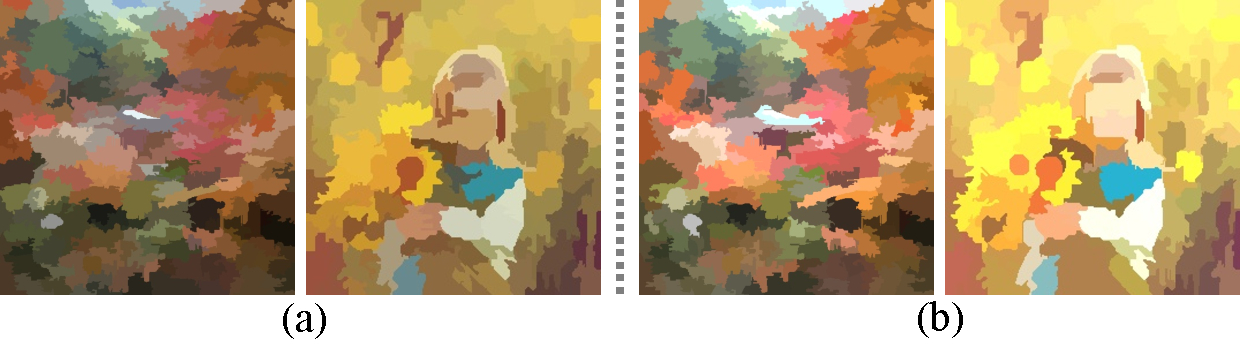
\includegraphics[width=\linewidth]{imgs/color_algorithm.pdf}
\caption{Adaptive coloring algorithm. (a) shows average colored segmentation map and (c) shows adaptively colored segmentation map, which are brighter and have higher contrast.}
\label{fig:color_algorithm}
\vspace{-0.5em}
\end{figure}

\begin{figure}[t]
\centering
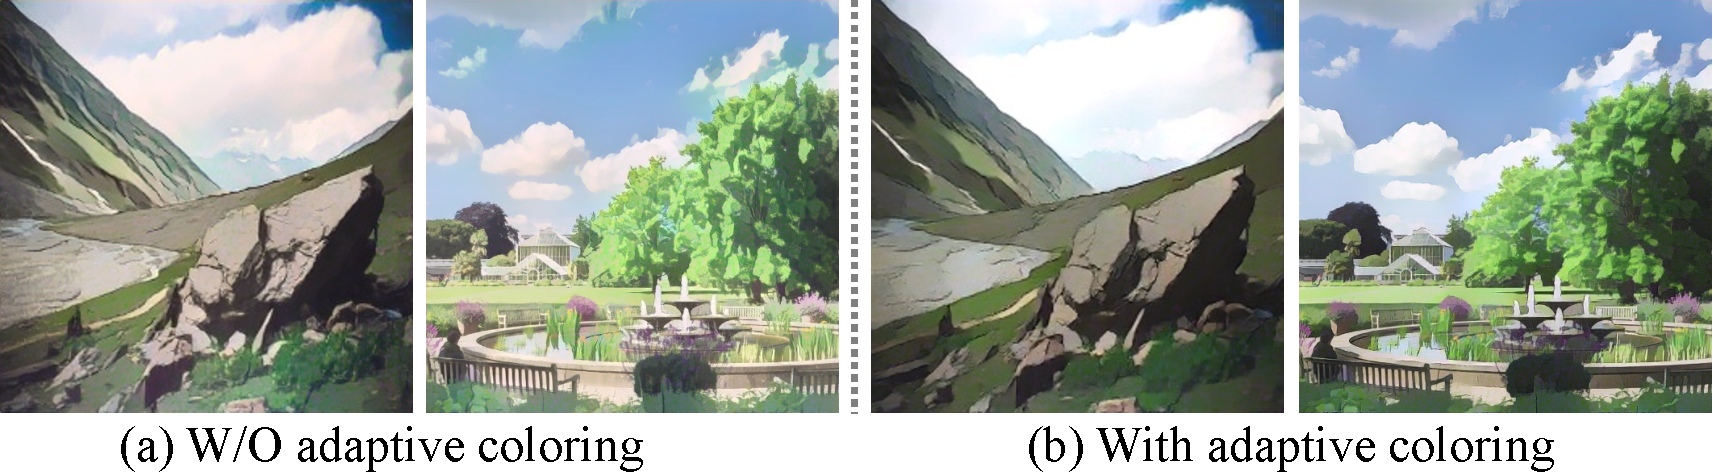
\includegraphics[width=\linewidth]{imgs/hazing.pdf}
\caption{Removal of hazing effect. (a) shows results trained with average colored structure representations, which suffer from hazing effects. (b) shows results trained with adaptively colored structure representations, which are brighter and free from hazing effects.}
\label{fig:hazing}
\vspace{-0.5em}
\end{figure}

\subsection{Learning From the Textural Representation}
The high-frequency features stored in cartoon images are desired as learning objectives, but luminance and color information make it easy to distinguish between cartoon images and real-world photos. We thus propose a random color shift algorithm $\mathcal{F}_{rcs}$ to extract single-channel texture representation from color images, which retains high-frequency texture information and helps avoid the influence of color and luminance.
\begin{equation}
\vspace{-0.3em}
\mathcal{F}_{rcs}(\bm{I}_{rgb}) = (1-\alpha)(\beta_1*\bm{I}_r + \beta2 *\bm{I}_g + \beta_3 *\bm{I}_b)+\alpha*\bm{Y}
\label{eqn:equation4}
%\vspace{-0.2em}
\end{equation}

In Equation \ref{eqn:equation4}, $\bm{I}_{rgb}$ represents 3-channel RGB color images, $\bm{I}_{r}, \bm{I}_{g}$ and $\bm{I}_{b}$ represent three color channels, and $\bm{Y}$ represents standard grayscale image converted from RGB color image. We set $\alpha=0.8$, $\beta_1$, $\beta_2$ and $\beta_3$ $\sim U(-1, 1)$. As is shown in Figure \ref{fig:framework}, the random color shift can generate random intensity maps with luminance and color information removed. A discriminator $\textit D_{t}$ is introduced to distinguish texture representations extracted from model outputs and cartoons, and guide the generator to learn the clear contours and fine textures stored in the texture representations. 
\begin{equation}
\vspace{-0.5em}
\begin{aligned}
\mathcal{L}_{texture}(\textit G, \textit D_{t}) &= log\textit D_{t}({\mathcal{F}_{rcs}}(\bm{I}_c))\\
&+log(1-\textit D_{t}(\mathcal{F}_{rcs}(\textit G(\bm{I}_p))))
\end{aligned}
\label{eqn:equation5}
%\vspace{-0.2em}
\end{equation}

\subsection{Full model}
Our full model is a GAN based framework with one generator and two discriminators. It is jointly optimized with features learned from three cartoon representations and could be formulated in Equation \ref{eqn:equation6}. By adjusting and balancing $\lambda_1$, $\lambda_2$, $\lambda_3$ and $\lambda_4$, it could be easily adapted to various applications with different artistic style. 
\begin{equation}
\begin{aligned}
\mathcal{L}_{total} &= \lambda_1*\mathcal{L}_{surface} + \lambda_2*\mathcal{L}_{texture} \\
&+ \lambda_3*\mathcal{L}_{structure} + \lambda_4*\mathcal{L}_{content} +\lambda_5*\mathcal{L}_{tv}
\end{aligned}
\label{eqn:equation6}
%\vspace{-0.2em}
\end{equation}

The total-variation loss $\mathcal{L}_{tv}$ \cite{aly2005image} is used to impose spatial smoothness on generated images. It also reduces high-frequency noises such as salt-and-pepper noise. In Equation \ref{eqn:equation7}, {\textit H, W, C} represent spatial dimensions of generated images. 
\begin{equation}
\begin{aligned}
\mathcal{L}_{tv} &= \frac{1}{H*W*C} \| \bigtriangledown_x({\textit G}(\bm{I}_p)) + \bigtriangledown_y({\textit G}(\bm{I}_p))\| 
\end{aligned}
\label{eqn:equation7}
\end{equation}
The content loss $\mathcal{L}_{content}$ is used to ensure that the cartoonized results and input photos are semantically invariant, and the sparsity of $\mathcal{L}_1$ norm allows for local features to be cartoonized. Similar to the structure loss, it is calculated on pre-trained VGG16 feature space:
\begin{equation}
\mathcal{L}_{content} = \| {\textit VGG_n}({\textit G}(\bm{I}_p)) - {\textit VGG_n}(\bm{I}_p)\|
\label{eqn:equation8}
\end{equation}

\subsection{Post processing and Style Interpolation}
\vspace{-0.3em}
To remove undesired high-frequency noises caused by adversarial training and maintain good perceptual quality, we use a differentiable guided filter $\mathcal{F}_{dgf}$ for post processing during training. Denote the network input as $\bm{I}_{in}$ and network output as $\bm{I}_{out}$, we formulated the post-processing in Equation \ref{eqn:equation9}, where $\bm{I}_{in}$ is used as guide map:
\begin{equation}
\vspace{-0.2em}
\bm{I}_{out} = \mathcal{F}_{dgf}(\bm{I}_{in}, \textit{G}(\bm{I}_{in}))
\label{eqn:equation9}
\vspace{-0.2em}
\end{equation}

We further find that, by interpolating the $\bm{I}_{out}$ and $\textit{G}(\bm{I}_{in})$, the sharpness of edges and details could be effectively tuned without having to fine-tune the network parameters. The interpolation is formulated in Equation \ref{eqn:equation10}, and the results of post-processing are shown in Figure \ref{fig:post_processing}.
\begin{equation}
\vspace{-0.5em}
\bm{I}_{interp} = \delta*\bm{I}_{out} + (1-\delta) * \textit{G}(\bm{I}_{in})
\label{eqn:equation10}
\vspace{-0.5em}
\end{equation}

\begin{figure}[t]
\centering
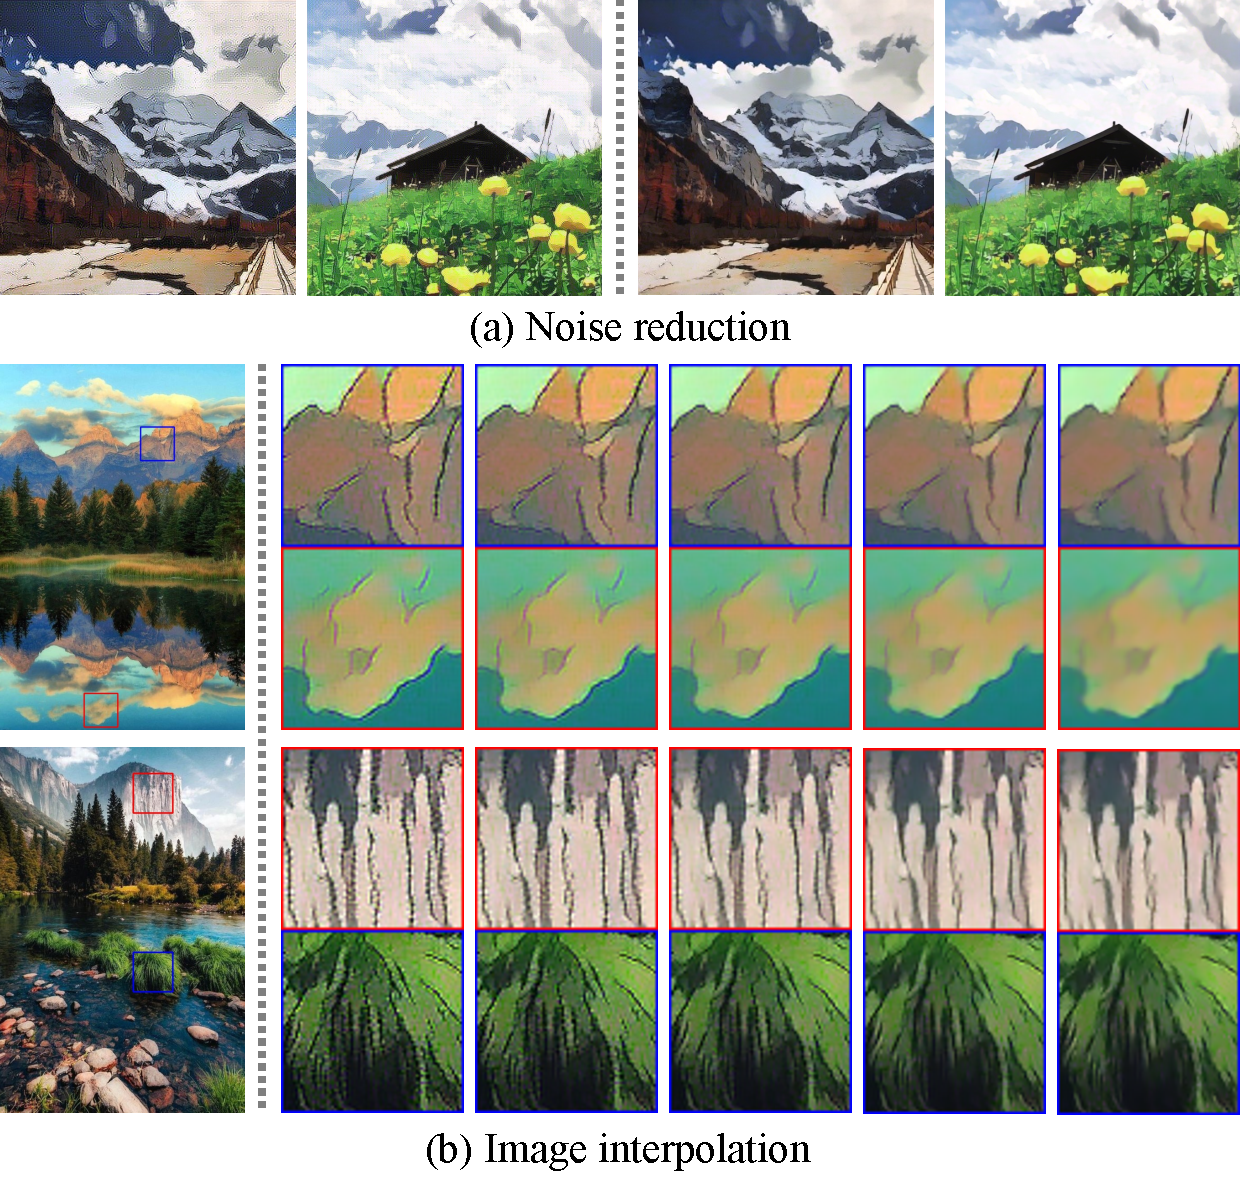
\includegraphics[width=\linewidth]{imgs/post_process.pdf}
\caption{Illustration of post-processing. (a) Our post processing can effectively turn noisy images(left) to clean images(right). (b) The sharpness of details could be adjusted. $\delta$ = 0.0, 0.25, 0.5, 0.75, 1.0 from left to right. Zoom in for details.}
\label{fig:post_processing}
\vspace{-1em}
\end{figure}

\begin{figure*}[t]
\centering
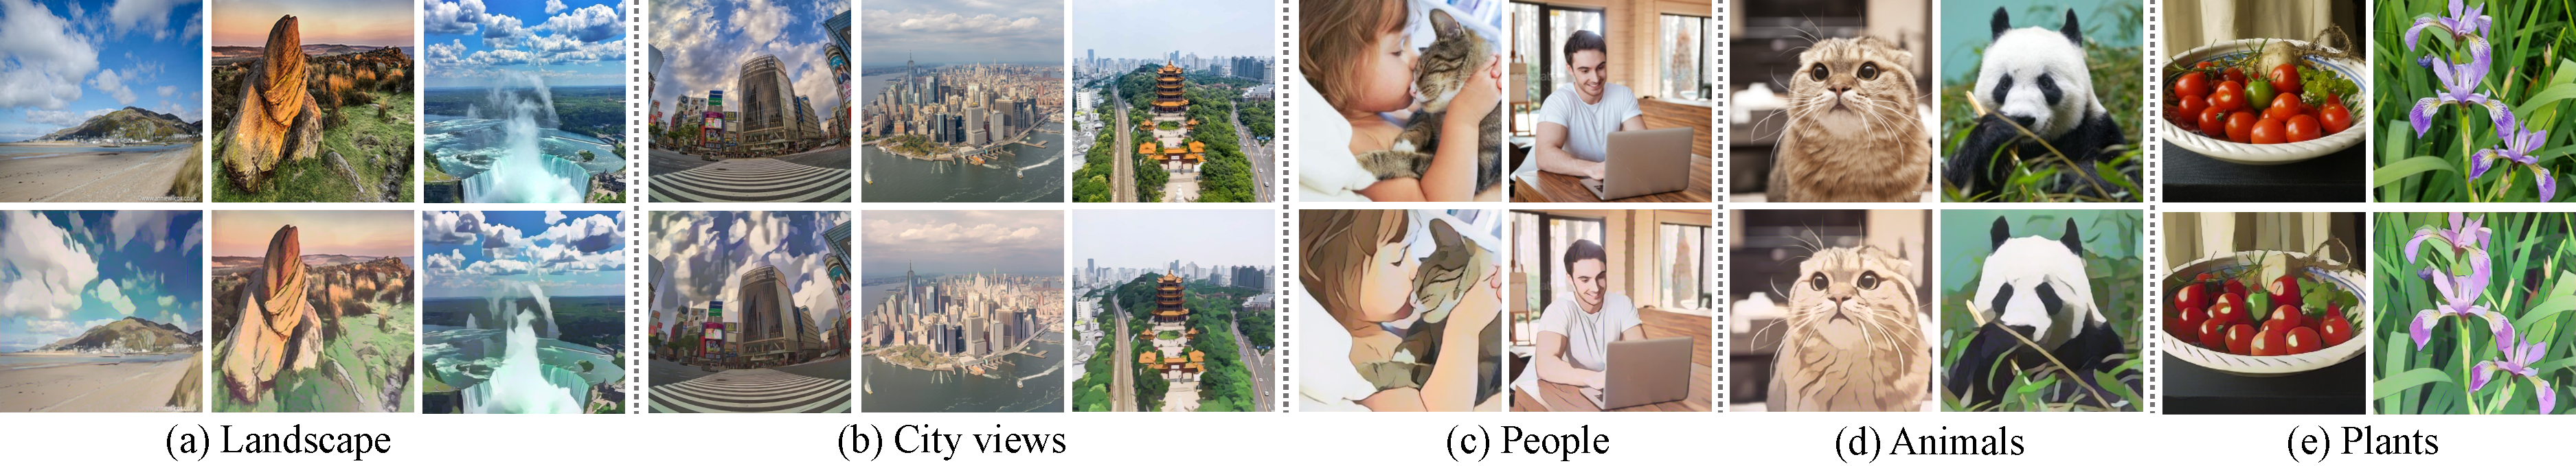
\includegraphics[width=\linewidth]{imgs/diverse_scenes.pdf}
\caption{Results of our method in different scenes. Zoom in for details}
\label{fig:diverse_scenes}
\vspace{-0.5em}
\end{figure*}

\begin{figure*}[htbp]
\centering
\includegraphics[width=\linewidth]{imgs/control.pdf}
\caption{Output quality could be controlled by adjusting weight of each representation. Zoom in for details.}
\label{fig:figure5}
\vspace{-0.5em}
\end{figure*}

\section{Experimental Results}
\vspace{-0.3em}
\subsection{Experimental Setup}
\vspace{-0.3em}
\textbf{Implementation.} We implement our GAN based framework with TensorFlow \cite{abadi2016tensorflow}. The generator and discriminator architectures are described in the supplementary material. Patch discriminator \cite{isola2017image} is adopted to simplify calculation and enhance discriminative capacity. We use Adam \cite{kingma2014adam} optimization algorithm to optimize both networks. Learning rate and batch size are set to $2*10^{-4}$ and 16 during training. For stability, we at first pre-train the generator with the content loss for 50000 iterations, and then jointly optimize the GAN based framework. Training is stopped when reaching 100000 iterations or on convergency. All results shown in this paper, unless specially mentioned, are generated with $\lambda_1=1, \lambda_2=10, \lambda_3=2*10^3, \lambda_4=2*10^3, \lambda_5=10^4$. 

\textbf{Dataset.} Both human face and landscape data are collected for generalization on diverse real-world scenes. For real-world photos, we collect 10000 images from the FFHQ dataset \cite{karras2019style} for the human face and 5000 images from the dataset in \cite{CycleGAN2017} for landscape. For cartoon images, we collect 10000 images from animations for the human face and 10000 images for landscape. Producers of collected animations include Kyoto animation, P.A.Works, Shinkai Makoto, Hosoda Mamoru, and Miyazaki Hayao. For validation set, we collect 3011 animation images and 1978 real-world photos. Images used in user study are collected from the Internet and Microsoft COCO \cite{lin2014microsoft} dataset. During training, all images are resized to 256*256 resolution, and face images are feed only once in every 5 iterations.

\textbf{Previous Methods.} We compare our method with three algorithms that represent Neural Style Transfer \cite{johnson2016perceptual}, Image-to-Image Translation \cite{CycleGAN2017} and Image Cartoonization \cite{chen2018cartoongan} respectively. For fair comparisons, We train CycleGAN and Fast Neural Style with the same training data and feeding schedule as our method, and set all the hyper-parameters by default or follow the author's recommendation. For CartoonGAN, we directly use the four official pre-trained models. 

\textbf{Evaluation metrics.} In qualitative experiments, we present results with details of four different methods and original images, as well as qualitative analysis. In quantitative experiments, we use Frechet Inception Distance (FID) \cite{heusel2017gans} to evaluate the performance by calculating the distance between source image distribution and target image distribution. In the user study, candidates are asked to rate results of different methods between 1 to 5 in cartoon quality and overall quality, higher scores mean better quality.

\begin{figure*}[htbp]
\centering
\includegraphics[width=\linewidth]{imgs/figure4.pdf}
\caption{Qualitative comparison of our method and previous methods. The Hosoda style, Shinkai style,  Hayao style and Paprika style of CartoonGAN \cite{chen2018cartoongan} are shown in row 1-4 respectively. Zoom in for details}
\label{fig:comparison}
\end{figure*}

\begin{table}[t]
\centering
\begin{tabular}{ccccc}
\hline
{Methods}&{\cite{johnson2016perceptual}}&{\cite{chen2018cartoongan}}&{\cite{CycleGAN2017}}&{Ours}\\
\hline  
{LR, CPU(ms)}&{639.31}&{1947.97}&{1332.66}&{\textbf{64.66}}\\
{LR, GPU(ms)}&{16.53}&{13.76}&{9.22}&{\textbf{3.58}}\\
{HR, GPU(ms)}&{48.96}&{148.02}&{106.82}&{\textbf{17.23}}\\
\hline 
{Parameter(M)}&{1.68}&{11.38}&{11.13}&{\textbf{1.48}}\\
\hline 
\end{tabular}
\caption{Performance and model size comparison, LR represents 256*256 resolution, while HR represents 720*1280 resolution}\label{table:speed}
\vspace{-1em}
\end{table}

\textbf{Time Performance and Model Size.} Speeds of four methods are compared on Intel i7-8750h CPU and Nvidia Tesla V-100 GPU. Shown in Table \ref{table:speed}, our model is the fastest among four methods on all devices and all resolutions, and has the smallest model size. It is worth mentioning that our model can process a 720*1280 image on GPU within only 17.23ms, which enables it for real-time High-Resolution video processing task at the speed of more than 50 FPS.

\textbf{Generality to diverse use cases.} We apply our model on diverse real-world scenes, including natural landscape, city views, people, animals, and plants, and show the results in Figure \ref{fig:diverse_scenes}. More examples of different styles and diverse use cases are shown in the supplementary material.

\vspace{-0.3em}
\subsection{Validation of Cartoon Representations.} 
\vspace{-0.3em}
To validate our proposed cartoon representations reasonable and effective, a classification experiment and a quantitative experiment based on FID are conducted, and the results are shown in Table \ref{table:prior}. We train a binary classifier on our training dataset to distinguish between real-world photos and cartoon images. The classifier is designed by adding a fully-connected layer to the discriminator in our framework. The trained classifier is then evaluated on the validation set to validate the influence of each cartoon representation. 

\begin{table}[t]
%\vspace{-1em}
\centering
\begin{tabular}{ccccc}
\hline
{No.}&{Surface}&{Structure}&{Texture}&{Original}\\
\hline  
{Acc}&{$0.8201$}&{0.6342}&{0.8384}&{0.9481}\\
\hline 
{FID}&{113.57}&{112.86}&{112.71}&{162.89}\\
\hline
\end{tabular}
\caption{Classification accuracy and FID evaluation of our proposed cartoon representation.}
\label{table:prior}
\vspace{-1em}
\end{table}

We find the extracted representations successfully fool the trained classifier, as it achieves lower accuracy in all three extracted cartoon representations compared to the original images. The calculated FID metrics also support our proposal that cartoon representations help close the gap between real-world photos and cartoon images, as all three extracted cartoon representations have smaller FID compared to the original images. 

\begin{table*}[t]
\centering
\begin{tabular}{cccccc}
\hline
{Methods}&{Photo}&{Fast Neural Style \cite{johnson2016perceptual}}&{CycleGAN \cite{CycleGAN2017}}&{CartoonGAN \cite{chen2018cartoongan}, average}&{Ours}\\
\hline  
{FID to Cartoon}&{162.89}&{146.34}&{141.50}&{130.38}&{\textbf{101.31}}\\
{FID to Photo}&{N/A}&{103.48}&{122.12}&{75.28}&{\textbf{28.79}}\\
\hline 
{Methods}&{Shinkai style of \cite{chen2018cartoongan}}
&{Hosoda style of \cite{chen2018cartoongan}}
&{Hayao style of \cite{chen2018cartoongan}}
&{Paprika style of \cite{chen2018cartoongan}}&{Ours}\\
\hline  
{FID to Cartoon}&{135.94}&{130.76}&{127.35}&{127.05}&{\textbf{101.31}}\\
%\hline 
{FID to Photo}&{37.96}&{58.13}&{86.48}&{118.56}&{\textbf{28.79}}\\
\hline 
\end{tabular}
\caption{Performance evaluation based on FID}\label{table:table1}
\vspace{-1em}
\end{table*}

\begin{figure*}[htb]
\centering
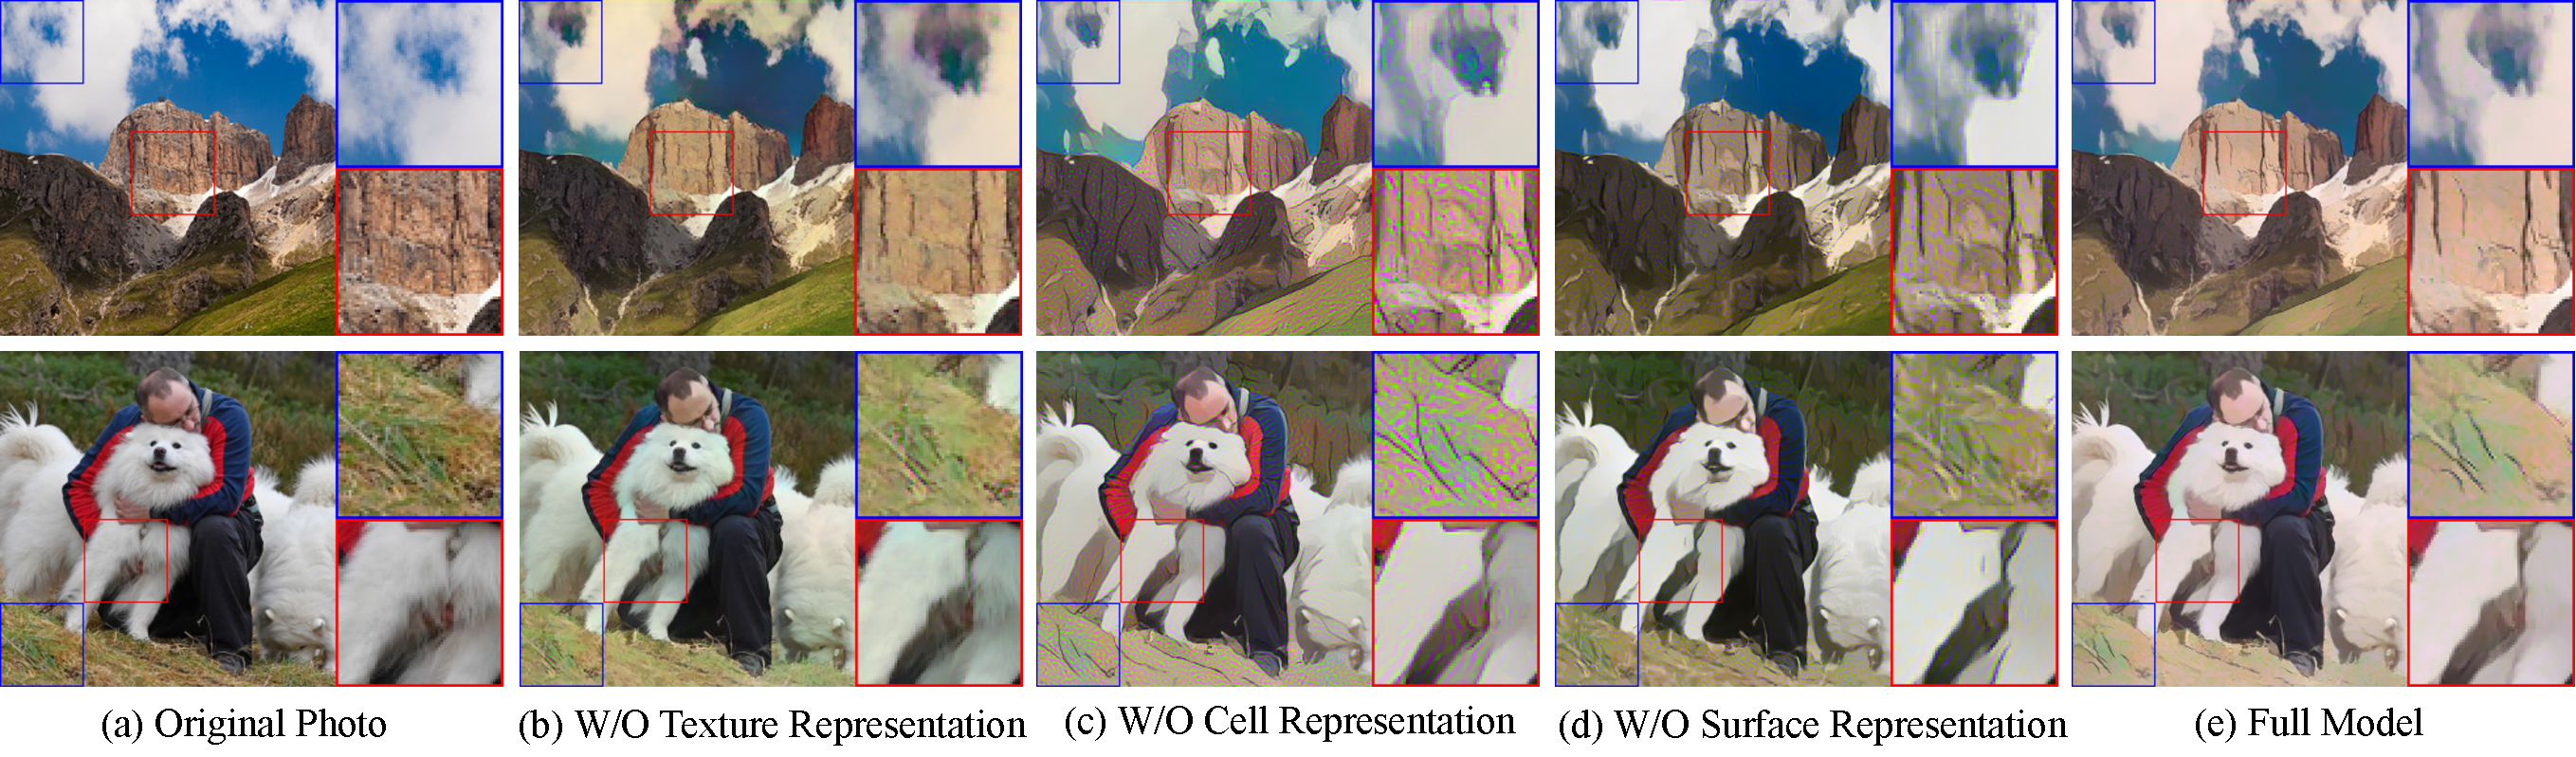
\includegraphics[width=\linewidth]{imgs/ablation_study.pdf}
\caption{Ablation study by removing each component}
\label{fig:figure7}
\vspace{-1em}
\end{figure*}

% user study or classifier results to show that after guided filtering, superpixel and random color shift, photos and cartoons are more difficult to be distinguished.
\vspace{-0.3em}
\subsection{Illustration of Controllability}
\vspace{-0.3em}
As is shown in Figure \ref{fig:figure5}, the style of cartoonized results could be adjusted by turning the weight of each representation in the loss function. Increase the weight of texture representation adds more details in the images. By setting $\lambda_2=20$, rich details such as plants on the wall and the contours of the house are preserved. This is because it regulates dataset distributions and enhances high-frequency details stored in texture representation. Smoother textures and fewer details are generated with a higher weight of surface representation. We setting $\lambda_1=2$ and $\lambda_2=10$, the details of the grassland and the mountain are smoothed. The reason is that guided filtering smooths training samples and reduces densely textured patterns. To get more abstract and sparse features, we can increase the weight of structure representation. By setting $\lambda_3=4*10^3~and~\lambda_4=6*10^3$, the details of the highway are abstracted into sparse color blocks. This is because the selective search algorithm flattens the training data and abstract them into structure representations. To conclude, unlike black-box models, our white-box method is controllable and can be easily adjusted.
\vspace{-0.3em}
\subsection{Qualitative Comparison}
\vspace{-0.3em}
Comparisons between our method and previous methods are shown in Figure \ref{fig:comparison}. The white-box framework helps keep global color harmonious. While all previous methods cause unrealistic color distortion like the green sky and brown clouds, our method effectively prevents improper color modification, such as clouds, sky, and mountains. Cartoon representations also help generate smooth features and sharp boundaries. CycleGAN causes distortions in sky and clouds, CartoonGAN generates distorted building details and messy mountain textures, whereas our method generates details with clear contours and smooth textures such as castles, mountains, and clouds. Lastly, our proposed representations effectively reduce high-frequency artifacts. Fast Neural Style suffers from pepper-and-salt noises and CycleGAN causes checkerboard artifacts, but our method generates noise-free images in all shown cases. To conclude, our method outperforms previous methods in generating images with harmonious color, cartoon-like features, clear boundaries, and fewer noises. More examples are shown in the supplementary materials.
\vspace{-0.3em}
\subsection{Quantitative Evaluation}
\vspace{-0.3em}
Frechet Inception Distance (FID) \cite{heusel2017gans} is a wildly-used metric to quantitatively evaluate the synthesizing performance of generative models. Pre-trained Inception-V3 model \cite{szegedy2016rethinking} is used to extract high-level features of images and calculate the distance between two image distributions. We use FID to evaluate the performance of previous methods and our method. As CartoonGAN models have not been trained on human face data, for fair comparisons, we only calculate FID on scenery dataset.

As is shown in Table \ref{table:table1}, our method generates images with smallest FID to cartoon image distribution. This proves that results generated by our method are most similar to the cartoon images. Output of our method also has smallest FID to real-world photo distribution, indicating that our method loyally preserves image content information.
\vspace{-0.3em}
\subsection{User Study}
\vspace{-0.3em}
The quality of Image cartoonization is highly subjective and greatly influenced by individual preference. We conducted user studies to show how users evaluate our method and previous methods. The user study involves 30 images, each processed by our proposed method and three previous methods. 10 candidates are asked to rate every image between 1-5 in 2 dimensions, following the criterion below:
%\newline 1.\textbf{Cartoon quality}: how do images look like cartoon image
%\newline 2.\textbf{Overall quality}: is there color shift, texture distortion, high-frequence noises, or other undesired artifacts
	\newline \textbf{Cartoon quality}: users are asked to evaluate how similar are the shown images and cartoon images.
	\newline \textbf{Overall quality}: users are asked to evaluate whether there are color shifts, texture distortions, high-frequency noises, or other artifacts they dislike on the images.

\begin{table}[t]
\centering
\begin{tabular}{ccccc}
\hline
{Methods}&{\cite{johnson2016perceptual}}&{\cite{chen2018cartoongan}}&{\cite{CycleGAN2017}}&{Ours}\\
\hline  
{Cartoon quality, mean}&{2.347}&{2.940}&{2.977}&{\textbf{4.017}}\\
{Cartoon quality, std}&{1.021}&{1.047}&{1.437}&{\textbf{0.962}}\\
\hline 
{Overall quality, mean}&{2.38}&{2.937}&{2.743}&{\textbf{3.877}}\\
{Overall quality, std}&{0.993}&{1.046}&{1.321}&{\textbf{0.982}}\\
\hline 
\end{tabular}
\caption{Result of User study, higher score means better quality. Row 1 and 2 represent the mean and standard error of Cartoon quality score, row 3 and 4 represent the mean and standard error of Overall quality score.}
\label{table:user_study}
\vspace{-1em}
\end{table}

We collect 1200 scores in total, and show the average score and standard error of each algorithm Table \ref{table:user_study}. Our method outperforms previous methods in both cartoon quality and overall quality, as we get higher scores in both criterions. This is because our proposed representations effectively extracted cartoon features, enabling the network to synthesis images with good quality. The synthesis quality of our method is also the most stable, as our method has the smallest standard error in both criterions. The reason is that our method is controllable and can be stabilized by balancing different components. Images used in user study are shown in the supplementary materials. 
\vspace{-0.3em}
\subsection{Analysis of Each Components}
\vspace{-0.3em}
We show the results of ablation studies in Figure \ref{fig:figure7}. Ablating the texture representation causes messy details. Shown in Figure \ref{fig:figure7}(a), irregular textures on the grassland and the dog's leg remains. This is due to the lack of high-frequency stored in the surface representation, which deteriorates the model's cartoonization ability. Ablating the structure representation causes high-frequency noises in Figure \ref{fig:figure7}(b). Severe pepper-and-salt appear on the grassland and the mountain. This is because the structure representation flattened images and removed high-frequency information. Ablating the surface representation causes both noise and messy details. Unclear edges of the cloud and noises on the grassland appear in Figure \ref{fig:figure7}(c). The reason is that guided filtering suppresses high-frequency information and preserves smooth surfaces. As a comparison, the results of our full model are shown in Figure \ref{fig:figure7}(d), which have smooth features, clear boundaries, and much less noise. In conclusion, all three representations help improve the cartoonizaiton ability of our method.
\vspace{-0.3em}
\section{Conclusion}
\vspace{-0.3em}
In this paper, we propose a white-box controllable image cartoonization framework based on GAN, which can generate high-quality cartoonized images from real-world photos. Images are decomposed into three cartoon representations: the surface representation, the structure representation, and the texture representation. Corresponding image processing modules are used to extract three representations for network training, and output styles could be controlled by adjusting the weight of each representation in the loss function. Extensive quantitative and qualitative experiments, as well as user studies, have been conducted to validate the performance of our method. Ablation studies are also conducted to demonstrate the influence of each representation.

\clearpage

{\small \bibliographystyle{ieee_fullname} \bibliography{egbib}}

\end{document}
